\documentclass[number]{autarticle}
\usepackage[utf8]{inputenc}
\usepackage{amsmath}
\usepackage{amsfonts}
\usepackage{amssymb}
\usepackage{graphicx}
\usepackage{caption , subcaption}
\usepackage{lipsum}
\usepackage{xcolor}
\usepackage{hyperref}
\usepackage{longtable}
\usepackage{booktabs}
\usepackage{array}
\usepackage{calc}
\graphicspath{{figures/}}
\newcommand{\SINR}{\mathrm{SINR}}

\begin{document}
\begin{frontmatter}

\title{AI-Enabled Beamforming and Dynamic Spectrum Allocation for Reliable Long-Range IoT over 6G}

\author{Mohammed Alabdullah}
\author{Vahid Amin-Ghafari}
\address[add1]{Iran University of Science and Technology, Computer Networks Engineering, Tehran, Iran}

\begin{abstract}
    Industrial environments expected in 6G will likely involve a mix of very different IIoT devices, including mobile robots such as AMRs and AGVs, alongside fixed sensors used for continuous monitoring of industrial operations. Integrating these diverse devices within the same industrial network remains challenging. Their operation depends on wireless links that can preserve reliability across longer coverage ranges while still meeting the demands of real-time control and ongoing data exchange. In practical settings, many existing scheduling and resource allocation schemes do not perform well enough, largely because they are built for more predictable network conditions than those found in dynamic industrial environments. The main issue is that they assume relatively stable conditions, while industrial networks are constantly changing due to varying traffic loads, device movement, and fluctuating channel quality. To address this challenge, this study explores the use of reinforcement learning (RL) for uplink scheduling in a conceptual 6G industrial setting. A reinforcement learning approach based on Proximal Policy Optimization (PPO) is used to decide how radio resources are shared between static sensors and mobile devices. Instead of following fixed rules, the agent is exposed to different traffic scenarios during training. This allows it to observe how congestion builds up and how different traffic types interact, gradually shaping its own scheduling strategy to keep the system operating in a stable manner. The simulation outcomes indicate that the PPO-based approach is capable of postponing the point at which system performance begins to degrade sharply, compared to a random scheduling strategy. This improvement is particularly noticeable for static sensing traffic, which achieves higher packet delivery ratios under moderate and heavy load conditions. However, as congestion intensifies, the learned policy tends to favor static devices, which leads to a noticeable drop in performance for AMR and AGV traffic. Under these conditions, an inversion behavior appears, where random scheduling can outperform PPO for mobile devices. Overall, the results highlight a clear trade-off when dealing with mixed industrial traffic types. They also underline the importance of designing scheduling mechanisms that explicitly account for mobility and multiple performance objectives. Future work can further improve these results by combining RL-based scheduling with advanced technologies such as AI-driven beamforming and digital twin systems to achieve more reliable and scalable industrial communication in emerging Industry 5.0 environments.
    
\end{abstract}

\begin{keywords}
6G \\
Industrial IoT \\
Industry 5.0 \\
Reliability \\
Constrained Reinforcement Learning \\
Proximal Policy Optimization \\
Dynamic Spectrum Allocation \\
Receive Beamforming \\
Deadline-Aware Scheduling \\
URLLC
\end{keywords}

\end{frontmatter}

\section{Introduction}\label{introduction}
Industrial wireless systems are moving toward mixed environments in which fixed sensors, automated guided vehicles (AGVs), autonomous mobile robots (AMRs), and other cyber-physical devices share the same radio infrastructure. Such systems must support high reliability and bounded latency while coping with mobility, changing traffic intensity, and time-varying propagation conditions \cite{saad2020vision6g,letaief2019roadmap6g}. URLLC and deterministic industrial communication further tighten the joint requirements on packet loss and delay \cite{popovski2018urllc,sasiain2025tsn}, while recent mobile-robot measurements show that maintaining high uplink throughput at low control latency remains difficult in realistic deployments \cite{kornacki2025ugv}.

Radio-resource control in this setting is a coupled problem. A scheduler must decide which device transmits, which subchannel it uses, what receive beam is applied at the access point, and which transmit-power level is selected. These decisions interact with queue occupancy, packet deadlines, stale channel information, and power limits. Conventional heuristics remain attractive because they are simple and interpretable, but their performance may deteriorate when several of these effects occur simultaneously. Reinforcement learning (RL) offers a different approach by learning a policy directly from the system state and the observed consequences of earlier actions \cite{luong2019drlsurvey,zappone2019modelai}.

This study develops and evaluates a constrained RL framework for joint scheduling, dynamic spectrum allocation, receive-beam selection, and discrete power control in an industrial uplink. The main contributions are:
\begin{enumerate}
\item a reproducible system model for six static sensors and two mobile AMR/AGV devices under a 3GPP Indoor-Factory channel;
\item a slot-level autoregressive PPO formulation with explicit reliability, deadline, queue-overflow, and average-power constraints;
\item a comparison with deadline-aware, channel-aware, random, and oracle baselines using matched seeds and seed-level statistical inference; and
\item an empirical analysis of the conditions under which beam selection affects link quality but does not become the dominant packet-reliability bottleneck.
\end{enumerate}

The results are not uniformly favourable to the learned methods. In the evaluated regime, Earliest-Deadline-First (EDF) remains the strongest reliability baseline, while the learned beam selector does not exceed chance-level accuracy under the available training budget. The learned policies do, however, operate at lower average transmit power than the greedy channel-aware heuristics. These findings expose a practical trade-off between reliability, power use, and learning complexity rather than a universal advantage for one control method.

\section{Related Work}\label{related-work}
Deep RL has been widely investigated for wireless scheduling and resource allocation \cite{luong2019drlsurvey}. Recent work includes PPO-based uplink scheduling for NOMA-URLLC \cite{robaglia2024nomappo}, actor--critic scheduling for resource-constrained multiclass traffic \cite{avranas2023constrained}, and network-aided offline RL for real-time wireless traffic \cite{wan2023naorl}. These studies establish the relevance of learning-based scheduling under delay and QoS constraints, but they do not combine the full scheduling, spectrum, beam, and power action considered here for a mixed static/mobile industrial population.

The constrained-control component builds on PPO \cite{schulman2017ppo} and on established constrained-RL mechanisms. Constrained Policy Optimization uses a trust-region formulation \cite{achiam2017cpo}; reward-constrained policy optimization uses a primal--dual Lagrangian mechanism \cite{tessler2019rcpo}; and PID-Lagrangian methods study responsive multiplier updates \cite{stooke2020pid}. The present method adopts a projected Lagrangian update for empirical episode-sum shortfalls without transferring theoretical convergence or safety guarantees from those works.

Joint spectrum and power decisions have also been studied with deep RL. Zhang et al. combined multi-agent learning for bandwidth and power allocation in the uplink \cite{zhang2023jointbw}, while Mismar et al. considered joint beamforming, power control, and interference coordination \cite{mismar2020drl5g}. Beam-management research has addressed mobility, beam training, and aged channel information in mmWave and emerging 6G systems \cite{heng2021beammanagement,xue2024beamsurvey,hussain2022beamtracking}. Industrial requirements and deterministic networking provide the application context \cite{ho2024urllc,sasiain2025tsn,kornacki2025ugv}.

Within the literature considered in this study, the remaining gap is the joint treatment of dynamic subchannel allocation, discrete power control, finite-codebook receive-beam selection under stale CSI, and deadline-constrained scheduling for a mixed static and AMR/AGV uplink. The contribution lies in this combination and in its constrained, seed-level evaluation rather than in any one component in isolation.

\section{System Model}\label{system-model}
Figure~\ref{fig:arch} illustrates the evaluated system.

\begin{figure}[htbp]
\centering
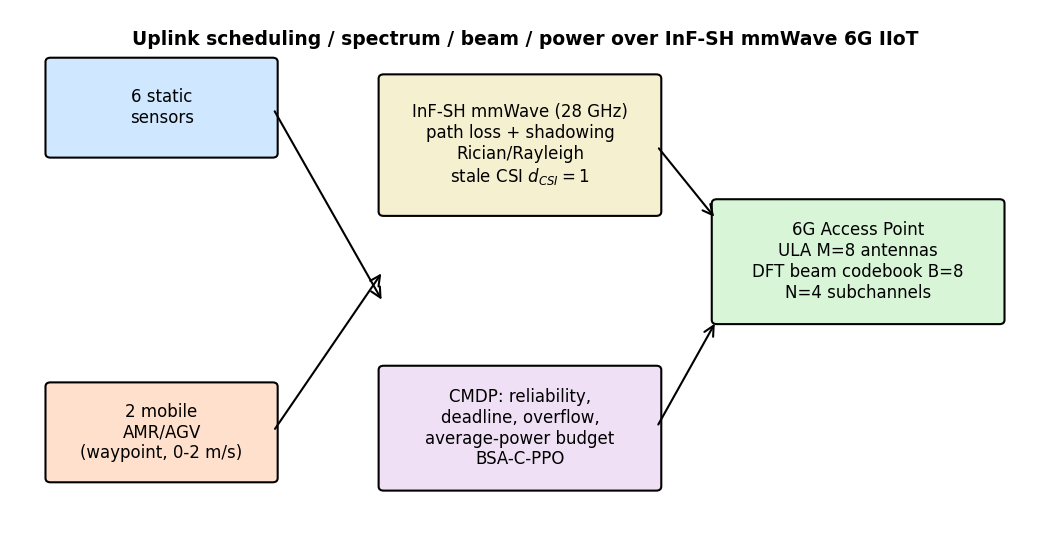
\includegraphics[width=0.88\linewidth]{fig1_architecture.png}
\caption{Industrial uplink model with static sensors, mobile AMR/AGV devices, four orthogonal subchannels, a finite receive-beam codebook, and discrete transmit-power control.}
\label{fig:arch}
\end{figure}

\subsection{Topology and physical layer}
A single access point equipped with an $M=8$ element uniform linear array serves $K=8$ uplink devices: six static sensors and two mobile AMR/AGV devices. The uplink provides $N=4$ orthogonal subchannels, with at most one user assigned to each subchannel in a slot. The number of devices therefore exceeds the number of simultaneously available subchannels, creating contention as load increases.

Each slot has duration $\tau=1$~ms and each subchannel has bandwidth $W=1$~MHz. The receiver noise figure is $NF=7$~dB and the thermal-noise variance is
\begin{equation}
\sigma_n^2=k_B T W 10^{NF/10}, \qquad T=290~\mathrm{K}.
\end{equation}
The receive codebook contains $B=8$ unit-norm DFT beams. Transmit power is selected from $\{0.05,0.10,0.20,0.40\}$~W, with a per-device total power cap of $0.8$~W. For device $k$, subchannel $n$, beam $b$, and power $p$, the instantaneous SINR is
\begin{equation}
\SINR_{k,n,b}=\frac{p\,\beta_{k,n}\,G_{k,n,b}}{\sigma_n^2},
\end{equation}
where $\beta_{k,n}$ is the large-scale path gain and $G_{k,n,b}=\lvert\mathbf{w}_b^{\mathsf H}\mathbf{h}_{k,n}\rvert^2$ is the receive-beam gain. A packet of $L$ bits is successfully delivered when
\begin{equation}
W\tau\log_2\!\left(1+\SINR_{k,n,b}\right)\ge L.
\end{equation}
Static packets are 256~bytes and mobile packets are 64~bytes, corresponding to required spectral efficiencies of 2.048 and 0.512~bit/s/Hz, respectively.

\subsection{Industrial channel and mobility}
Large-scale propagation follows the 3GPP TR~38.901 Indoor-Factory Sparse-clutter High-BS (InF-SH) model \cite{tr38901}. For LOS links,
\begin{equation}
PL_{\mathrm{LOS}}=31.84+21.50\log_{10}(d_{3D})+19.00\log_{10}(f_c),
\end{equation}
with $f_c$ in GHz. For InF-SH NLOS links,
\begin{align}
PL'_{\mathrm{SH}} &= 32.4+23.0\log_{10}(d_{3D})+20.0\log_{10}(f_c),\\
PL_{\mathrm{SH}} &= \max\left(PL'_{\mathrm{SH}},PL_{\mathrm{LOS}}\right).
\end{align}
Shadow-fading standard deviations are 4~dB for LOS and 5.9~dB for InF-SH NLOS. The LOS probability follows the corresponding InF-SH exponential form, with the subscenario parameter obtained from the selected clutter geometry. The primary carrier frequency is 28~GHz.

The small-scale channel uses a correlated Rician model for LOS and a correlated Rayleigh model for NLOS. This is a beam-level abstraction rather than a full clustered TR~38.901 channel realization. Mobile devices follow seeded, grid-constrained piecewise-linear trajectories inside the factory hall at speeds up to 2~m/s. Beam decisions are made from channel information delayed by one slot.

\subsection{Traffic, queues, and reliability}
Packet arrivals are independent Bernoulli processes with offered-load probability
$p\in\{0.05,0.10,0.20,0.30,0.40\}$ per device per slot. Static and mobile queues are FIFO with capacities of 32 and 16 packets. Their packet deadlines are 10 and 2 slots, and their retransmission limits are 3 and 1, respectively. Each evaluation episode contains $T_{\mathrm{meas}}=200$ measurement slots followed by a drain phase in which new arrivals are disabled and remaining cohort packets are served until every packet reaches a terminal delivered or dropped state.

The empirical delivery floors are 0.99 for static traffic and 0.995 for mobile traffic. The $10^{-5}$ URLLC loss level is treated as a standards reference rather than as a quantity that can be certified by a finite ten-seed simulation.

\subsection{CMDP formulation}
The action in a physical slot is a sequence of $N$ conditional tokens. The constraints comprise reliability, deadline-violation, and queue-overflow shortfalls for each traffic class, together with a measurement-window average-power shortfall. For class $c$,
\begin{equation}
C_{\mathrm{rel},c}=\sum_t\left(\rho_c a_{c,t}-d_{c,t}\right),
\end{equation}
where $a_{c,t}$ and $d_{c,t}$ are generated and delivered cohort packets, respectively. The power constraint is
\begin{equation}
C_{\mathrm{pow}}=\sum_{t\in\mathcal{W}_{\mathrm{meas}}}\left(P_t-\bar P\right),\qquad \bar P=0.80~\mathrm{W}.
\end{equation}
All shortfalls are feasible when their episode sums are non-positive.

\begin{table}[t]\centering\small
\caption{Frozen confirmatory scenario parameters.}\label{tab:scenario}
\begin{tabular}{@{}p{0.30\columnwidth}p{0.62\columnwidth}@{}}\toprule
Parameter & Value \\ \midrule
Access point & ULA, $M=8$ antennas, single cell (OMA) \\
Devices & 6 static sensors + 2 mobile AMR/AGV ($K=8$) \\
Subchannels & $N=4$ orthogonal; beam codebook $B=8$ (DFT) \\
Carrier / bandwidth & $f_c=28$ GHz; $W=1$ MHz per subchannel \\
Slot / noise figure & $\tau=1$ ms; $NF=7$ dB; $T=290$ K \\
Power levels & $P\in\{0.05,0.10,0.20,0.40\}$ W; $P_{\max}=0.4$ W \\
Power budget & $\bar P=0.80$ W (sensitivity 0.64/0.80/0.96) \\
Channel & 3GPP TR 38.901 InF-SH; Rician/Rayleigh ULA \\
Deadlines & static 10 / mobile 2 slots; retx 3 / 1 \\
Queues & static 32 / mobile 16 packets (FIFO) \\
Packet size & static 256 B / mobile 64 B \\
Offered load grid & $p\in\{0.05,0.10,0.20,0.30,0.40\}$; $p_{\mathrm{ref}}=0.20$ \\
Measurement horizon & $T_{\mathrm{meas}}=200$ slots + full drain \\
Stale CSI & $d_{\mathrm{CSI}}=1$ slot \\
Confirmatory seeds & $\{20001,\dots,20010\}$ ($n=10$, fresh) \\
Training budget & 8 episodes $\times$ 10 updates, hidden 48 (bounded) \\
\bottomrule\end{tabular}\end{table}

\section{Proposed BSA-C-PPO}\label{proposed-method}
The policy constructs one joint action per slot through an autoregressive decoder. At decoder step $n$, the token specifies either idle or a device--beam--power combination for the current subchannel. A conditional mask removes actions that violate subchannel exclusivity, packet availability, per-device allocation limits, or power caps before sampling. The environment independently validates the final joint action and rejects an infeasible action rather than repairing it after the fact.

The policy therefore produces one joint slot log-probability and one PPO probability ratio per physical slot. The constrained variant, BSA-C-PPO, uses one reward critic and one shared vector cost critic with
\begin{equation}
J_{\mathrm{cost}}=3\lvert\mathcal{C}\rvert+1=7
\end{equation}
outputs. The ordered cost channels are static reliability, deadline, and overflow; mobile reliability, deadline, and overflow; and the average-power shortfall.

The Lagrangian advantage is
\begin{equation}
A_t^{L}=A_t^{\mathrm{reward}}-
\sum_{i=1}^{J_{\mathrm{cost}}}\lambda_i s_i A_t^{\mathrm{cost},i},
\end{equation}
where $s_i$ is a fixed scaling factor. Multipliers are updated once per training batch using
\begin{equation}
\lambda_i\leftarrow\left[\lambda_i+\eta_{\lambda,i}s_i\widehat{C}_i\right]_+.
\end{equation}
The cost channel uses $\gamma_{\mathrm{cost}}=1$ and $\lambda_{\mathrm{cost}}=0.95$. The reward used in the final evaluation combines successful delivery, head-of-line age, and subchannel utilisation. Unconstrained and fixed-penalty PPO variants use the same network and action construction so that differences can be attributed to the constraint mechanism rather than to a different action space.

\section{Experimental Setup}\label{experimental-setup}
The final evaluation used a fixed scenario and analysis plan before outcome analysis. Calibration runs used only seeds 10001--10003. Primary inference used ten fresh seeds, 20001--20010, matched across methods and evaluated at the five offered-load points. The primary comparison consisted of 12 methods, 10 seeds, and 5 loads, yielding 600 method--load--seed records. Secondary analyses examined CSI delay, power budget, channel correlation, clutter height, and token order.

Layer~1 isolates scheduling under fixed radio settings and compares Fixed-Radio Random with Fixed-Radio Base PPO. Layer~2 evaluates Random, Round Robin, EDF, Stale-Max-Gain, current-CSI Max-SINR, a perfect-current-CSI beam oracle, Last-Beam, BSA-Unconstrained-PPO, BSA-Penalty-PPO, and BSA-C-PPO in the full action space.

The learning implementation used a bounded CPU training budget of 8 rollout episodes per update for 10 updates with a hidden dimension of 48. This budget was sufficient to execute the full protocol reproducibly but did not produce reliable beam learning. That limitation is considered explicitly when interpreting the learned-policy results.

Seed is the statistical unit for inference. Matched-seed comparisons use paired differences across the ten primary seeds. The analysis reports mean effects, 95\% confidence intervals, paired tests, effect sizes, and Holm adjustment for multiple primary comparisons where applicable. Pooled packet ratios are used descriptively and are not treated as independent inferential replicates.

\section{Results}\label{results}
\subsection{Reliability under increasing load}
Figure~\ref{fig:pdr} shows packet delivery as offered load increases. EDF provides the strongest reliability in the tested regime and maintains a mobile PDR of 1.000 at all five load levels. At $p=0.40$, BSA-C-PPO reaches a mobile PDR of 0.959 and a static PDR of 0.993. The difference in mobile PDR relative to EDF is $-0.041$; the matched-seed comparison gives Holm-adjusted $p=0.039$ and Cohen's $d_z=-0.85$.

\begin{figure}[htbp]
\centering
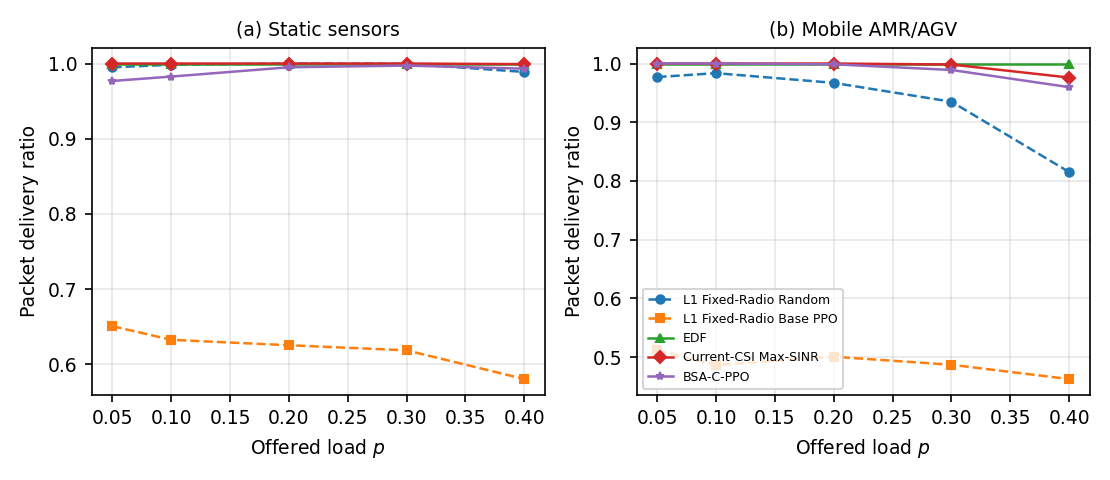
\includegraphics[width=0.82\linewidth]{fig2_pdr_vs_load.png}
\caption{Packet delivery ratio as a function of offered load for selected methods.}
\label{fig:pdr}
\end{figure}

The fixed-radio Layer~1 comparison did not reproduce an advantage for Base PPO over Random. At the highest load, Fixed-Radio Random achieves static and mobile PDRs of 0.989 and 0.815, whereas Fixed-Radio Base PPO reaches 0.575 and 0.458. This result is consistent with insufficient policy learning under the available training budget and shows that the benefit of PPO cannot be assumed when a well-matched scheduling baseline is available.

\subsection{Latency and congestion}
The mobile deadline is only two slots, making service order critical when $K>N$. EDF addresses this directly and therefore remains difficult to improve upon. Figure~\ref{fig:lat} shows the p95 latency trend. The learned policies remain usable at moderate load but lose reliability as the high-load region is approached.

\begin{figure}[htbp]
\centering
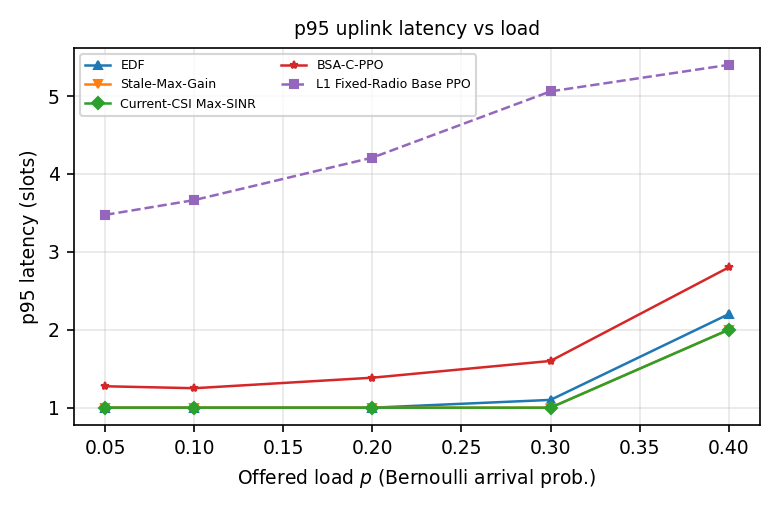
\includegraphics[width=0.82\linewidth]{fig3_latency_vs_load.png}
\caption{p95 uplink latency across the offered-load sweep.}
\label{fig:lat}
\end{figure}

\subsection{Beam selection}
Beam-optimal heuristics reach high agreement with the current-CSI oracle, but this does not translate into a reliability advantage over EDF. Figure~\ref{fig:beam} compares beam-selection accuracy with the chance reference $1/B=0.125$. BSA-C-PPO remains below or close to chance across the load sweep, whereas the channel-aware heuristics track the oracle closely.

\begin{figure}[htbp]
\centering
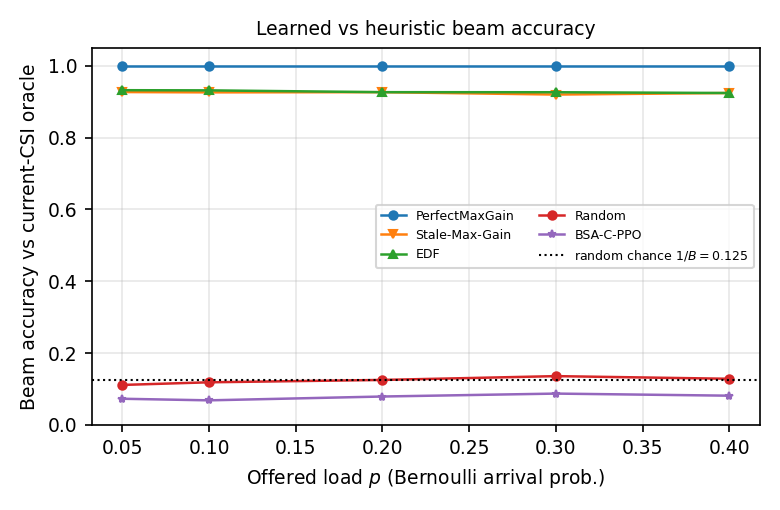
\includegraphics[width=0.82\linewidth]{fig5_beam_acc_vs_load.png}
\caption{Beam-selection accuracy relative to the current-CSI oracle. The horizontal reference is random chance, $1/B=0.125$.}
\label{fig:beam}
\end{figure}

This finding does not imply that receive-beam alignment is irrelevant. The channel-aware methods obtain higher beam gain and spectral efficiency. In this topology, however, deadline-aware service order has a larger effect on packet delivery than beam choice.

\subsection{Power use and constraint behaviour}
Figure~\ref{fig:power} shows average transmit power. At $p=0.40$, the learned policies operate at about 0.60~W, below the 0.80~W budget, while EDF and the greedy channel-aware methods operate near 1.28~W. The lower average power is an empirical property of the learned policy family under the evaluated reward and training configuration. It cannot be attributed specifically to the Lagrangian mechanism because the constrained, fixed-penalty, and unconstrained PPO variants are not measurably separated in the primary evaluation.

\begin{figure}[htbp]
\centering
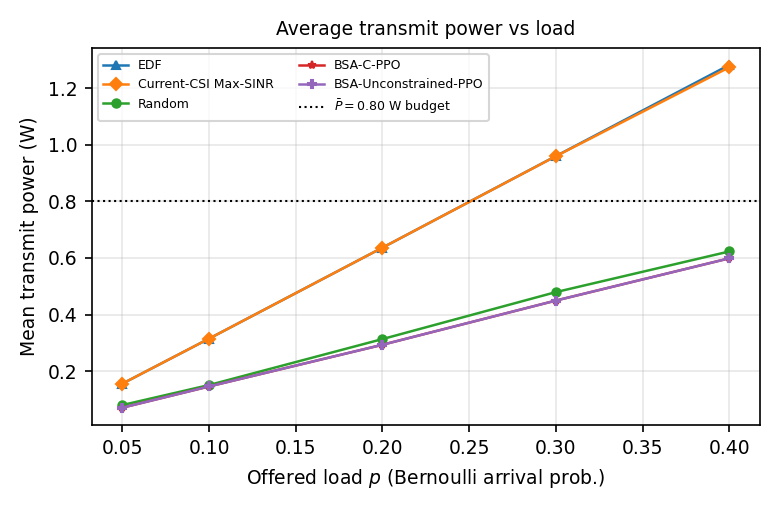
\includegraphics[width=0.82\linewidth]{fig4_power_vs_load.png}
\caption{Mean transmit power versus offered load. The dashed reference marks the $\bar P=0.80$~W average-power budget.}
\label{fig:power}
\end{figure}

For BSA-C-PPO, the fraction of seeds satisfying all constraints decreases as load rises and reaches 0.1 at $p=0.40$ (Fig.~\ref{fig:feas}). The main limiting constraint shifts toward mobile reliability in the most congested region.

\begin{figure}[htbp]
\centering
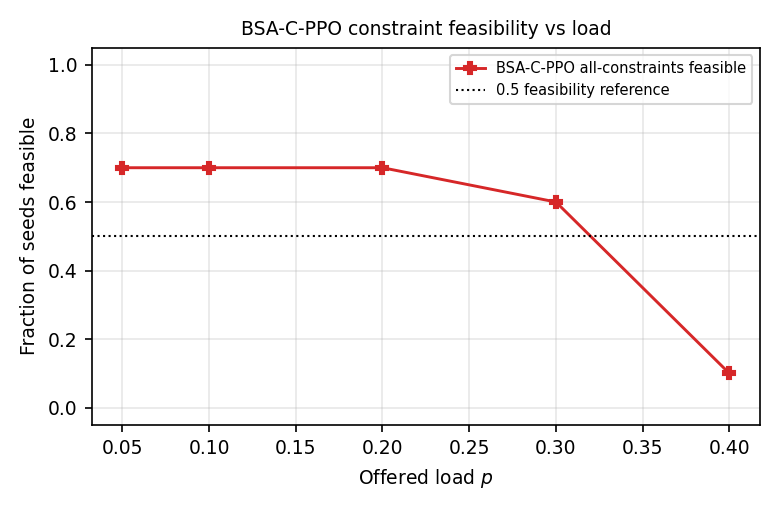
\includegraphics[width=0.82\linewidth]{fig6_feasibility_vs_load.png}
\caption{Fraction of BSA-C-PPO seeds satisfying all empirical constraints at each offered-load point.}
\label{fig:feas}
\end{figure}

\subsection{Learning behaviour}
The three PPO variants produce effectively identical primary metrics under the available training budget. At $p=0.40$, BSA-C-PPO and BSA-Unconstrained-PPO have the same mobile PDR (0.959), with a paired difference of 0.000 and adjusted $p=1.000$. The multipliers respond to constraint violations, but the resulting changes are not large enough to produce a distinct policy within the evaluated training horizon.

\begin{figure}[htbp]
\centering
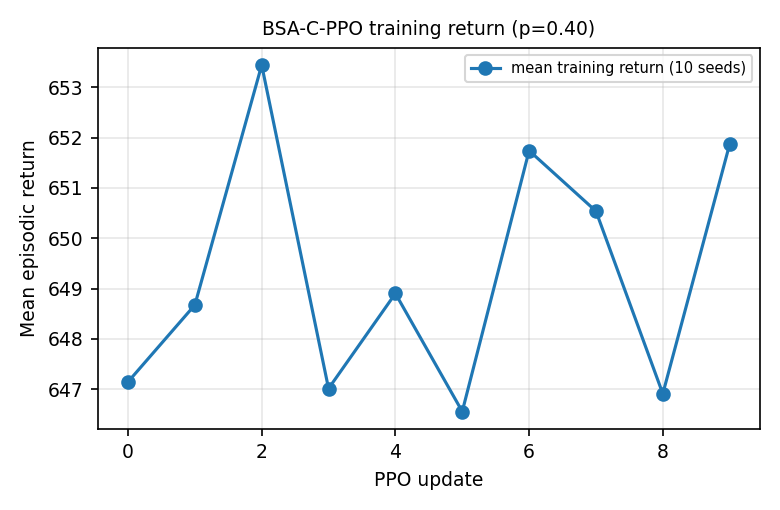
\includegraphics[width=0.82\linewidth]{fig7_training_curve.png}
\caption{Mean episodic BSA-C-PPO training return at $p=0.40$ across the ten evaluation seeds.}
\label{fig:train}
\end{figure}

\begin{table*}[t]\centering\small
\caption{Confirmatory results at peak load $p=0.40$ (seed-mean, $n=10$). PDR = packet delivery ratio; power in W; beam accuracy vs the current-CSI oracle (random chance $=0.125$).}\label{tab:p40}
\begin{tabular}{@{}lccccc@{}}\toprule
Method & PDR (static) & PDR (mobile) & p95 latency (slots) & Mean power (W) & Beam accuracy \\ \midrule
EDF & 1.000 & 1.000 & 2.2 & 1.282 & 0.924 \\
Max-SINR oracle & 0.999 & 0.976 & 2.0 & 1.274 & 1.000 \\
Stale-Max-Gain & 1.000 & 0.980 & 2.0 & 1.276 & 0.924 \\
Random & 1.000 & 0.967 & 2.6 & 0.623 & 0.128 \\
BSA-Uncon.-PPO & 0.993 & 0.959 & 2.8 & 0.599 & 0.081 \\
BSA-C-PPO & 0.993 & 0.959 & 2.8 & 0.599 & 0.081 \\
L1 Fixed Random & 0.989 & 0.815 & 6.5 & 1.235 & 0.135 \\
L1 Fixed Base PPO & 0.575 & 0.458 & 5.4 & 0.706 & 0.127 \\
\bottomrule\end{tabular}\end{table*}
\begin{table}[t]\centering\small
\caption{Matched-seed paired comparisons of BSA-C-PPO mobile PDR at $p=0.40$ ($n=10$; sign-flip permutation, Holm-adjusted).}\label{tab:stats}
\begin{tabular}{@{}lccc@{}}\toprule
Comparison (BSA-C-PPO $-$ B) & mean diff & Holm $p$ & $d_z$ \\ \midrule
vs EDF & -0.041 & 0.039 & -0.85 \\
vs BSA-Unconstrained-PPO & 0.000 & 1.000 & 0.00 \\
\bottomrule\end{tabular}\end{table}
\begin{table}[t]\centering\small
\caption{Accepted-abstract Layer-1 hypotheses evaluated on fresh confirmatory data.}\label{tab:hyp}
\begin{tabular}{@{}cp{0.40\columnwidth}p{0.40\columnwidth}@{}}\toprule
\# & Hypothesis & Verdict \\ \midrule
1 & Base PPO outperforms Random for static sensors & Not supported (Base-PPO static PDR 0.58--0.65 vs Random $\approx$1.00) \\
2 & Congestion degradation begins at a finite load & Supported (mobile PDR $<0.99$ from $p=0.05$) \\
3 & Mobile AMR/AGV degrade earlier than static & Supported \\
4 & A load exists where Random beats Base PPO for mobile (inversion) & Supported (all loads) \\
\bottomrule\end{tabular}\end{table}

\section{Discussion}\label{discussion}
The results show that a strong domain heuristic can outperform a substantially more flexible learned controller when the dominant system bottleneck is simple and clearly exposed. In this case, the two-slot mobile deadline makes service order critical. EDF responds directly to that structure and achieves perfect mobile delivery in the evaluated load range, whereas the learned controller must discover the same priority from reward feedback in a much larger action space.

Beam selection has a different role. Better beam alignment improves SINR and spectral efficiency, but packet reliability is often already limited by congestion and deadline expiry before beam gain becomes decisive. This explains why Stale-Max-Gain and the current-CSI oracle achieve high beam accuracy without surpassing EDF in packet delivery. The result should therefore be interpreted as regime-dependent: beam control is likely to matter more in coverage-limited or interference-limited deployments than in the single-cell OMA configuration studied here \cite{heng2021beammanagement,xue2024beamsurvey}.

The power results reveal another trade-off. The learned policies operate at substantially lower average transmit power than the greedy heuristics, but this comes with a small loss of reliability at the highest load. Because all three PPO variants behave almost identically, the experiment does not support attributing the lower power to the Lagrangian constraint mechanism itself. A larger training budget or a setting in which the power constraint binds more persistently may be necessary to separate these behaviours.

The study also highlights the limits of finite-sample reliability evaluation. The $10^{-5}$ URLLC order is useful as a standards reference, but a ten-seed simulation of this size cannot establish such a rare-event probability. The empirical delivery floors used here are therefore operational thresholds for comparative evaluation rather than certification targets.

\section{Limitations}\label{limitations}
Several limitations define the scope of the conclusions. First, the policy was trained with a CPU-limited budget in a 257-action space, and the learned beam selector remained near chance. The reported learned-policy performance should therefore be interpreted as compute-bounded rather than asymptotic. Second, the small-scale channel is a correlated beam-level abstraction and does not reproduce the full clustered TR~38.901 channel. Third, the evaluation considers a single-cell OMA system with no inter-cell or co-channel interference and one InF-SH topology. Fourth, the inferential sample comprises ten seeds, which is adequate for paired method comparisons but not for rare-event reliability certification. Finally, the present experiments do not establish a theoretical feasibility or safety guarantee for the constrained policy.

Future work should examine larger training budgets and stronger function approximators, richer industrial topologies with interference and handover, and additional coverage-limited regimes in which beam alignment directly controls packet success. Larger-scale reliability studies are also required before conclusions can be extended toward rare-event URLLC targets.

\section{Conclusion}\label{conclusion}
This paper examined joint scheduling, dynamic spectrum allocation, receive-beam selection, and power control for a mixed static/mobile industrial uplink. The proposed BSA-C-PPO formulation provides a unified constrained action model and was evaluated against strong scheduling, channel-aware, and oracle baselines using matched seeds across five offered loads.

The main result is that added control flexibility does not automatically improve reliability. EDF is the strongest reliability method in the tested regime because packet deadlines, rather than beam alignment, dominate the delivery outcome. Learned beam selection remains near chance under the available training budget, and the constrained PPO variant does not measurably separate from its unconstrained counterpart. At the same time, the learned policies operate at a considerably lower average transmit power than the greedy heuristics, revealing a measurable power--reliability trade-off.

These findings suggest that learning-based radio control should be evaluated against strong problem-specific heuristics and under multiple operating regimes. In industrial systems, the value of beamforming, constrained RL, and joint optimization depends on which physical or queueing mechanism actually limits service reliability.

\section{Data Availability}\label{data-availability}
The scenario configuration, evaluation protocol, source code, random seeds, seed-level records, and the logs and scripts used to reproduce the reported figures and tables are archived with the study materials. They can be made available in accordance with the applicable publication policy and author approval.

\begin{thebibliography}{99}\small
\bibitem{saad2020vision6g} W.~Saad, M.~Bennis, and M.~Chen, ``A Vision of 6G Wireless Systems: Applications, Trends, Technologies, and Open Research Problems,'' \emph{IEEE Network}, vol.~34, no.~3, pp.~134--142, 2020. doi:10.1109/MNET.001.1900287.
\bibitem{letaief2019roadmap6g} K.~B. Letaief, W.~Chen, Y.~Shi, J.~Zhang, and Y.-J.~A. Zhang, ``The Roadmap to 6G: AI Empowered Wireless Networks,'' \emph{IEEE Communications Magazine}, vol.~57, no.~8, pp.~84--90, 2019. doi:10.1109/MCOM.2019.1900271.
\bibitem{popovski2018urllc} P.~Popovski \emph{et al.}, ``Wireless Access for Ultra-Reliable Low-Latency Communication: Principles and Building Blocks,'' \emph{IEEE Network}, vol.~32, no.~2, pp.~16--23, 2018. doi:10.1109/MNET.2018.1700258.
\bibitem{sasiain2025tsn} J.~Sasiain, D.~Franco, A.~Atutxa, J.~Astorga, and E.~Jacob, ``Toward the Integration and Convergence Between 5G and TSN Technologies and Architectures for Industrial Communications: A Survey,'' \emph{IEEE Communications Surveys \& Tutorials}, vol.~27, no.~1, pp.~259--321, 2025. doi:10.1109/COMST.2024.3422613.
\bibitem{kornacki2025ugv} J.~Kornacki, A.~Wójcikowska, and M.~Hoeft, ``Meeting Industrial 5G Requirements for High Uplink Throughput and Low Control Latency in UGV Scenarios,'' \emph{Applied Sciences}, vol.~15, no.~12, art.~6427, 2025. doi:10.3390/app15126427.
\bibitem{luong2019drlsurvey} N.~C. Luong \emph{et al.}, ``Applications of Deep Reinforcement Learning in Communications and Networking: A Survey,'' \emph{IEEE Communications Surveys \& Tutorials}, vol.~21, no.~4, pp.~3133--3174, 2019. doi:10.1109/COMST.2019.2916583.
\bibitem{robaglia2024nomappo} B.-M. Robaglia, M.~Coupechoux, and D.~Tsilimantos, ``Deep Reinforcement Learning for Uplink Scheduling in NOMA-URLLC Networks,'' \emph{IEEE Transactions on Machine Learning in Communications and Networking}, vol.~2, pp.~1142--1158, 2024. doi:10.1109/TMLCN.2024.3437351.
\bibitem{avranas2023constrained} A.~Avranas, P.~Ciblat, and M.~Kountouris, ``Deep Reinforcement Learning for Resource Constrained Multiclass Scheduling in Wireless Networks,'' \emph{IEEE Transactions on Machine Learning in Communications and Networking}, vol.~1, pp.~225--241, 2023. doi:10.1109/TMLCN.2023.3314705.
\bibitem{wan2023naorl} J.~Wan, S.~Lin, Z.~Zhang, J.~Zhang, and T.~Zhang, ``Scheduling Real-Time Wireless Traffic: A Network-Aided Offline Reinforcement Learning Approach,'' \emph{IEEE Internet of Things Journal}, vol.~10, no.~24, pp.~22331--22340, 2023. doi:10.1109/JIOT.2023.3304969.
\bibitem{schulman2017ppo} J.~Schulman, F.~Wolski, P.~Dhariwal, A.~Radford, and O.~Klimov, ``Proximal Policy Optimization Algorithms,'' arXiv:1707.06347, 2017. doi:10.48550/arXiv.1707.06347.
\bibitem{achiam2017cpo} J.~Achiam, D.~Held, A.~Tamar, and P.~Abbeel, ``Constrained Policy Optimization,'' in \emph{Proc.\ 34th Int.\ Conf.\ Machine Learning (ICML)}, PMLR~70, pp.~22--31, 2017.
\bibitem{tessler2019rcpo} C.~Tessler, D.~J. Mankowitz, and S.~Mannor, ``Reward Constrained Policy Optimization,'' in \emph{Int.\ Conf.\ Learning Representations (ICLR)}, 2019.
\bibitem{stooke2020pid} A.~Stooke, J.~Achiam, and P.~Abbeel, ``Responsive Safety in Reinforcement Learning by PID Lagrangian Methods,'' in \emph{Proc.\ 37th Int.\ Conf.\ Machine Learning (ICML)}, PMLR~119, pp.~9133--9143, 2020.
\bibitem{zhang2023jointbw} C.~Zhang, T.~Lv, P.~Huang, Z.~Lin, J.~Zeng, and Y.~Ren, ``Joint Optimization of Bandwidth and Power Allocation in Uplink Systems with Deep Reinforcement Learning,'' \emph{Sensors}, vol.~23, no.~15, art.~6822, 2023. doi:10.3390/s23156822.
\bibitem{mismar2020drl5g} F.~B. Mismar, B.~L. Evans, and A.~Alkhateeb, ``Deep Reinforcement Learning for 5G Networks: Joint Beamforming, Power Control, and Interference Coordination,'' \emph{IEEE Transactions on Communications}, vol.~68, no.~3, pp.~1581--1592, 2020. doi:10.1109/TCOMM.2019.2961332.
\bibitem{heng2021beammanagement} Y.~Heng \emph{et al.}, ``Six Key Challenges for Beam Management in 5.5G and 6G Systems,'' \emph{IEEE Communications Magazine}, vol.~59, no.~7, pp.~74--79, 2021. doi:10.1109/MCOM.001.2001184.
\bibitem{xue2024beamsurvey} Q.~Xue \emph{et al.}, ``A Survey of Beam Management for mmWave and THz Communications Towards 6G,'' \emph{IEEE Communications Surveys \& Tutorials}, vol.~26, no.~3, pp.~1520--1559, 2024. doi:10.1109/COMST.2024.3361991.
\bibitem{hussain2022beamtracking} M.~Hussain and N.~Michelusi, ``Learning and Adaptation for Millimeter-Wave Beam Tracking and Training: A Dual Timescale Variational Framework,'' \emph{IEEE Journal on Selected Areas in Communications}, vol.~40, no.~1, pp.~37--53, 2022. doi:10.1109/JSAC.2021.3126086.
\bibitem{ho2024urllc} T.~M. Ho, K.-K. Nguyen, and M.~Cheriet, ``Energy Efficiency Deep Reinforcement Learning for URLLC in 5G Mission-Critical Swarm Robotics,'' \emph{IEEE Transactions on Network and Service Management}, vol.~21, no.~5, pp.~5018--5032, 2024. doi:10.1109/TNSM.2024.3406350.
\bibitem{zappone2019modelai} A.~Zappone, M.~Di Renzo, and M.~Debbah, ``Wireless Networks Design in the Era of Deep Learning: Model-Based, AI-Based, or Both?,'' \emph{IEEE Transactions on Communications}, vol.~67, no.~10, pp.~7331--7376, 2019. doi:10.1109/TCOMM.2019.2924010.
\bibitem{naik2020coexistence6ghz} G.~Naik, J.-M. Park, J.~Ashdown, and W.~Lehr, ``Next Generation Wi-Fi and 5G NR-U in the 6 GHz Bands: Opportunities and Challenges,'' \emph{IEEE Access}, vol.~8, pp.~153027--153056, 2020. doi:10.1109/ACCESS.2020.3016036.
\bibitem{tr38901} ETSI/3GPP, ``Study on channel model for frequencies from 0.5 to 100 GHz,'' 3GPP TR~38.901 version 18.1.0 Release~18 (ETSI TR~138\,901 V18.1.0), 2026-02-16.
\end{thebibliography}

\end{document}
